\documentclass[aspectratio=169]{beamer}
\usepackage[utf8]{inputenc}

\usetheme{default}
\usecolortheme{seahorse}
\setbeamertemplate{navigation symbols}{}

\AtBeginSection[]
{
    \begin{frame}
        \frametitle{Table of Contents}
        \tableofcontents[currentsection]
    \end{frame}
}

\setbeamertemplate{section in toc}[sections numbered]
\setbeamertemplate{subsection in toc}[subsections numbered]

\title{Introduction to Scientific Computing and Data Science}
\subtitle{Scientific Computing}
\author{Stefan Abi-Karam}
\date{Summer 2023}


\begin{document}

\begin{frame}
    \titlepage
\end{frame}


\section{Course Overview}

\begin{frame}{Course Goals}

    \begin{itemize}
        \item Overview of topics in \textbf{scientific computing}, \textbf{data science}, and \textbf{machine learning}
        \item Apply these topics to your own research
        \item Familiarize yourself with the tools and software
    \end{itemize}
\end{frame}

\begin{frame}{Course Survey}

    % two col
    \begin{columns}[t]
        \begin{column}{0.5\textwidth}
            \textbf{Topics}
            \begin{itemize}
                \item Programming Foundations
                \item Computer Science and Math Foundations
                \item Overview of Scientific Computing
                \item Exploratory Data Science and Visualization
                \item Machine Learning
                \item Deep Learning
            \end{itemize}
        \end{column}
        \begin{column}{0.5\textwidth}
            \textbf{Tools}
            \begin{itemize}
                \item Python
                \item NumPy, SciPy, Pandas
                \item Matplotlib, Seaborn
                \item Scikit-Learn, Scikit-Image
                \item PyTorch
            \end{itemize}
        \end{column}
    \end{columns}

\end{frame}

\begin{frame}{Course Logistics}
    Refer to the current year's course syllabus for more details.

    \vspace{\baselineskip}

    We will typically split the class into the following components:
    \begin{itemize}
        \item Lectures: Twice a week
        \item Homework: Once a week
        \item Office Hours: Typically once a week with demand
    \end{itemize}

    \vspace{\baselineskip}

    Grading is typically split as follows:
    \begin{itemize}
        \item Homework: $80\%$
        \item Participation + Other: $20\%$
    \end{itemize}
\end{frame}

\begin{frame}{Communication}

    \begin{itemize}
        \item Email: \href{mailto:stefan.abi-karam@ahschool.com}{stefan.abi-karam@ahschool.com}
              \begin{itemize}
                  \item Absence, Personal Concerns, Project Questions and Feedback
                  \item Please use your Heritage email address as well
              \end{itemize}

        \item Google Classroom
              \begin{itemize}
                  \item \textbf{Homework Assignments}
                  \item Class meeting link
                  \item Class announcements and changes
              \end{itemize}

        \item Campuswire
              \begin{itemize}
                  \item \textbf{Questions about Homework}
              \end{itemize}

        \item Office Hours
              \begin{itemize}
                  \item \textbf{Questions about Homework}
                  \item \textbf{Questions about Projects}
              \end{itemize}

        \item Slack
              \begin{itemize}
                  \item Project Questions and Feedback, Quick Updates, Meeting Links and Reminders
              \end{itemize}
    \end{itemize}

\end{frame}

\section{About Your Teacher}


\begin{frame}{About Your Teacher}

    \begin{itemize}
        \item Graduated from American Heritage in 2018
        \item B.S. in Electrical Engineering in 2021
        \item M.S. in Electrical Engineering in 2022
        \item Ph.D. + Research Faculty 2023 and beyond
    \end{itemize}

    \textbf{Research}: My research is focused on hardware acceleration of machine learning algorithms and applied machine learning for hardware design tools and emerging technologies.

    \vspace{\baselineskip}

    % three images in one row
    \begin{columns}[t]
        \begin{column}{0.33\textwidth}
            \centering
            \includegraphics[width=0.8\textwidth]{imgs/me_0.jpg}
        \end{column}
        \begin{column}{0.33\textwidth}
            \centering
            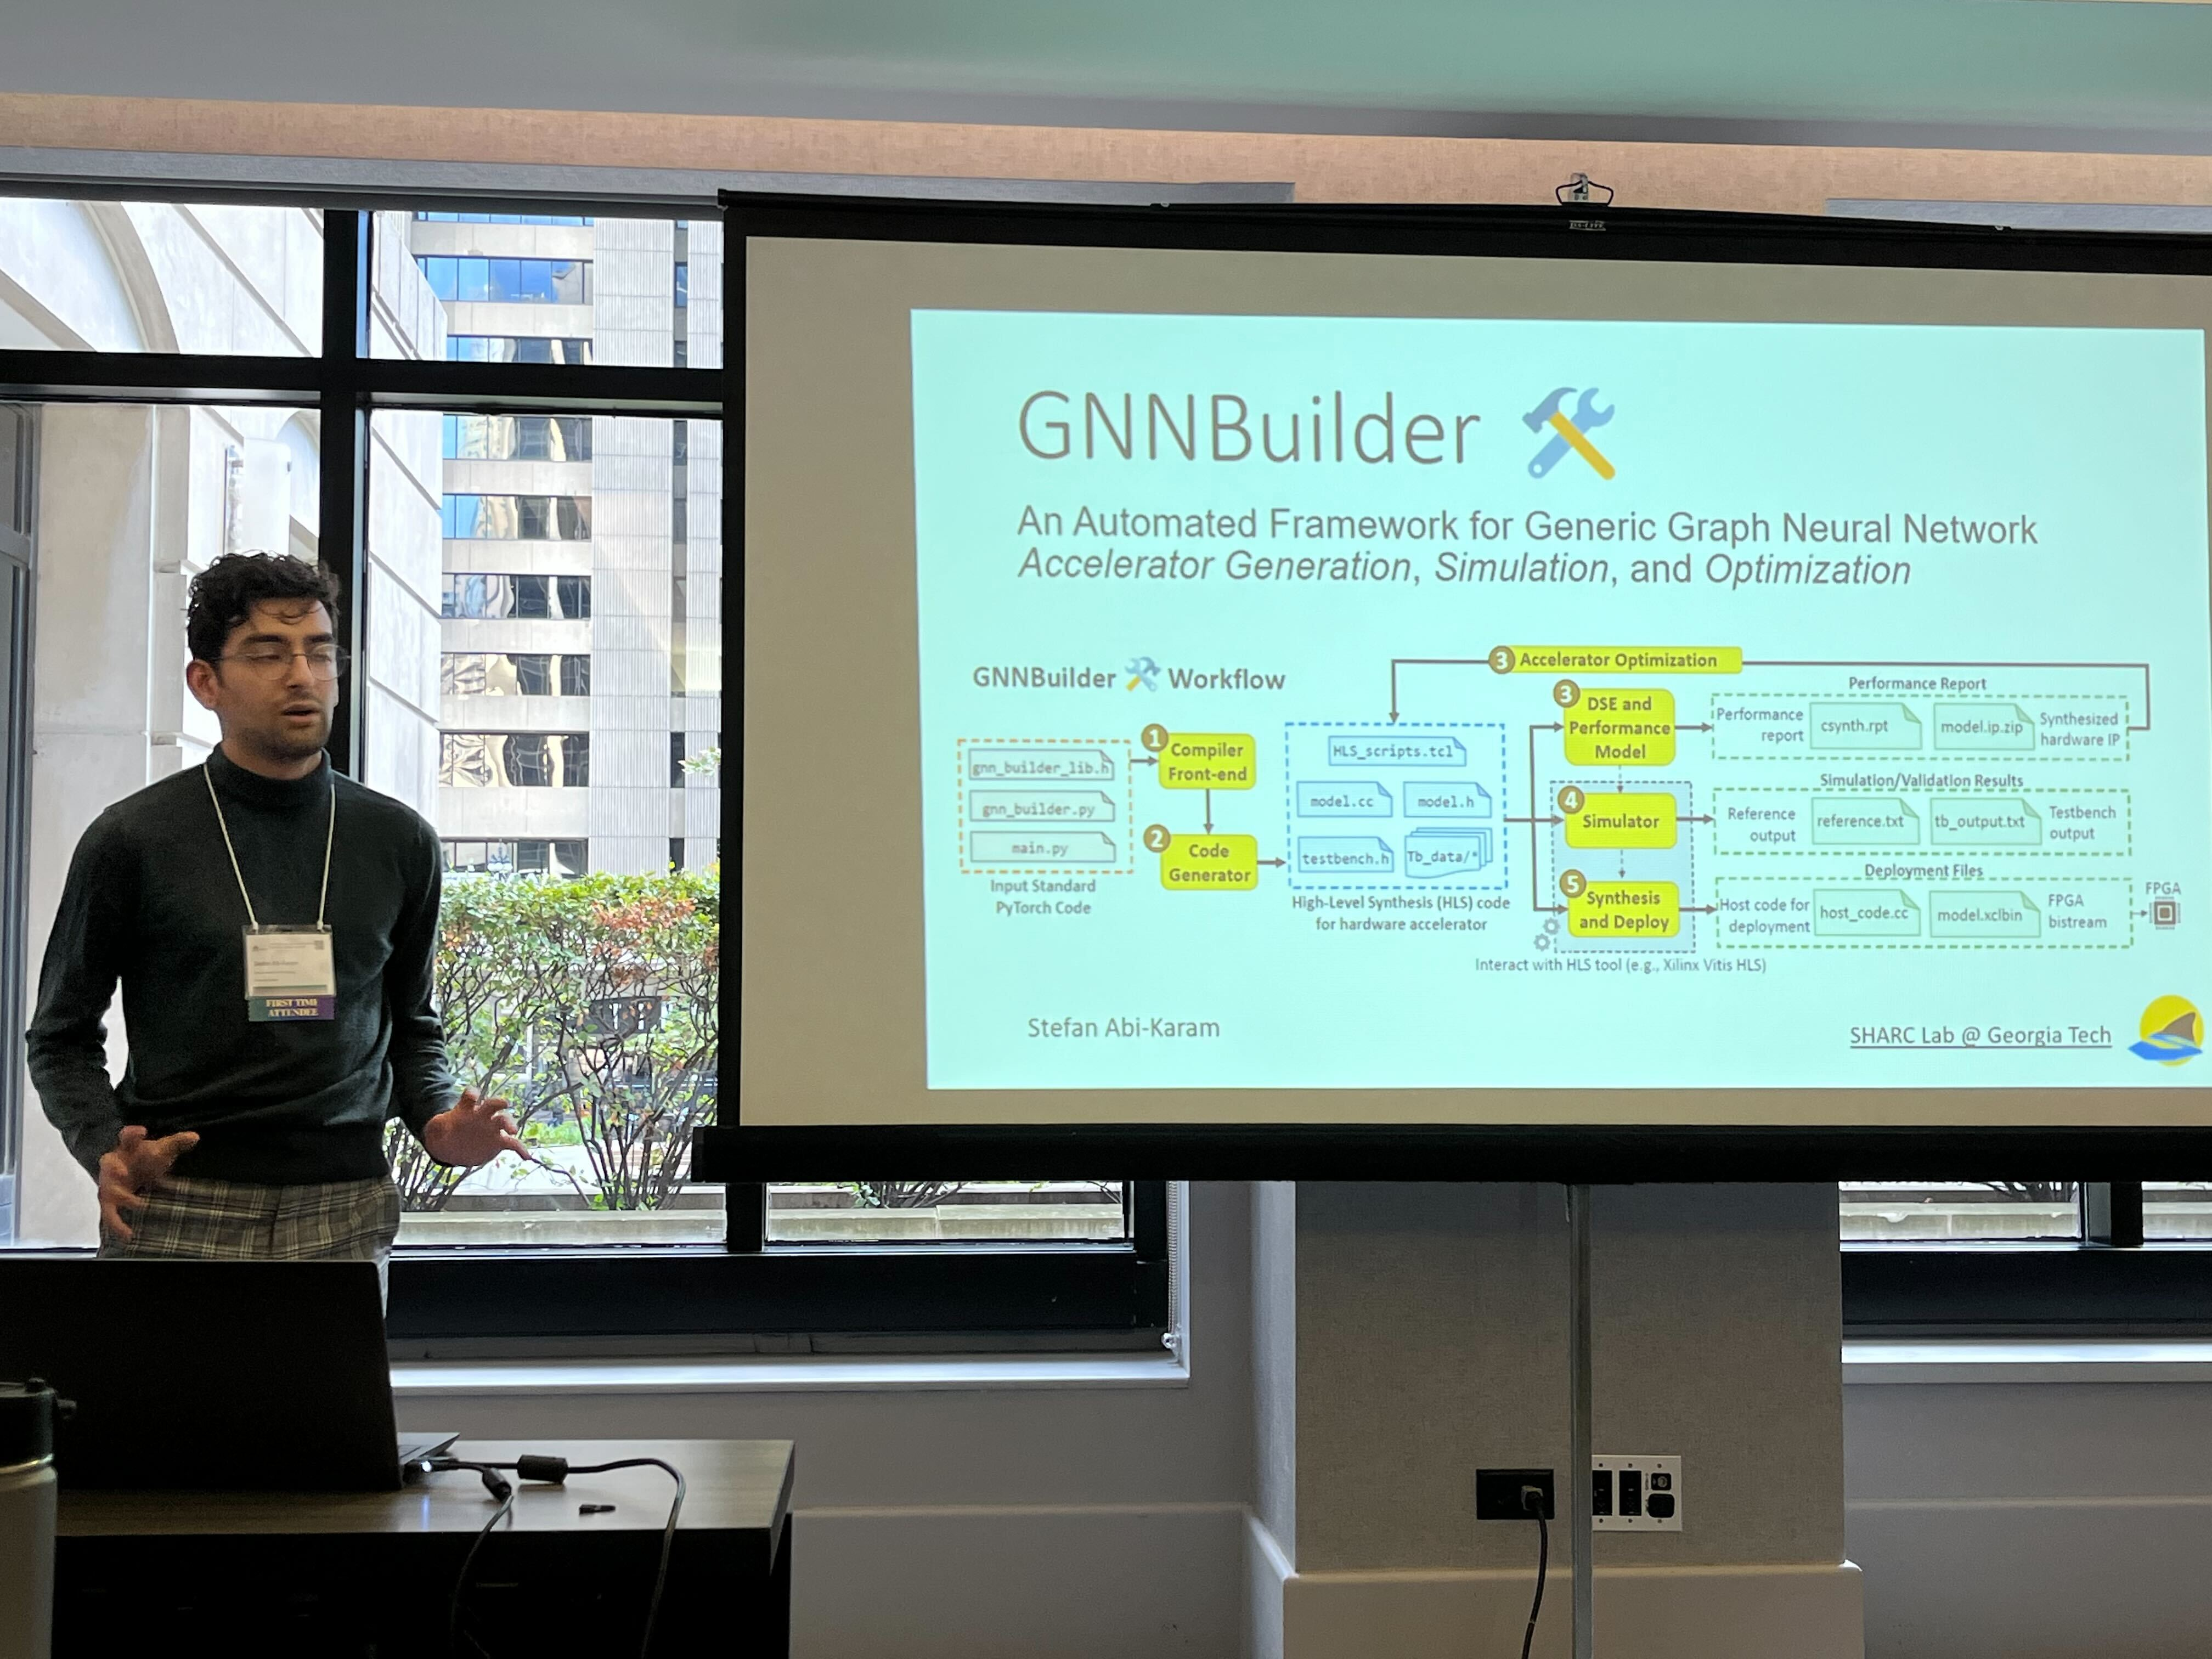
\includegraphics[width=0.8\textwidth]{imgs/me_1.jpg}
        \end{column}
        \begin{column}{0.33\textwidth}
            \centering
            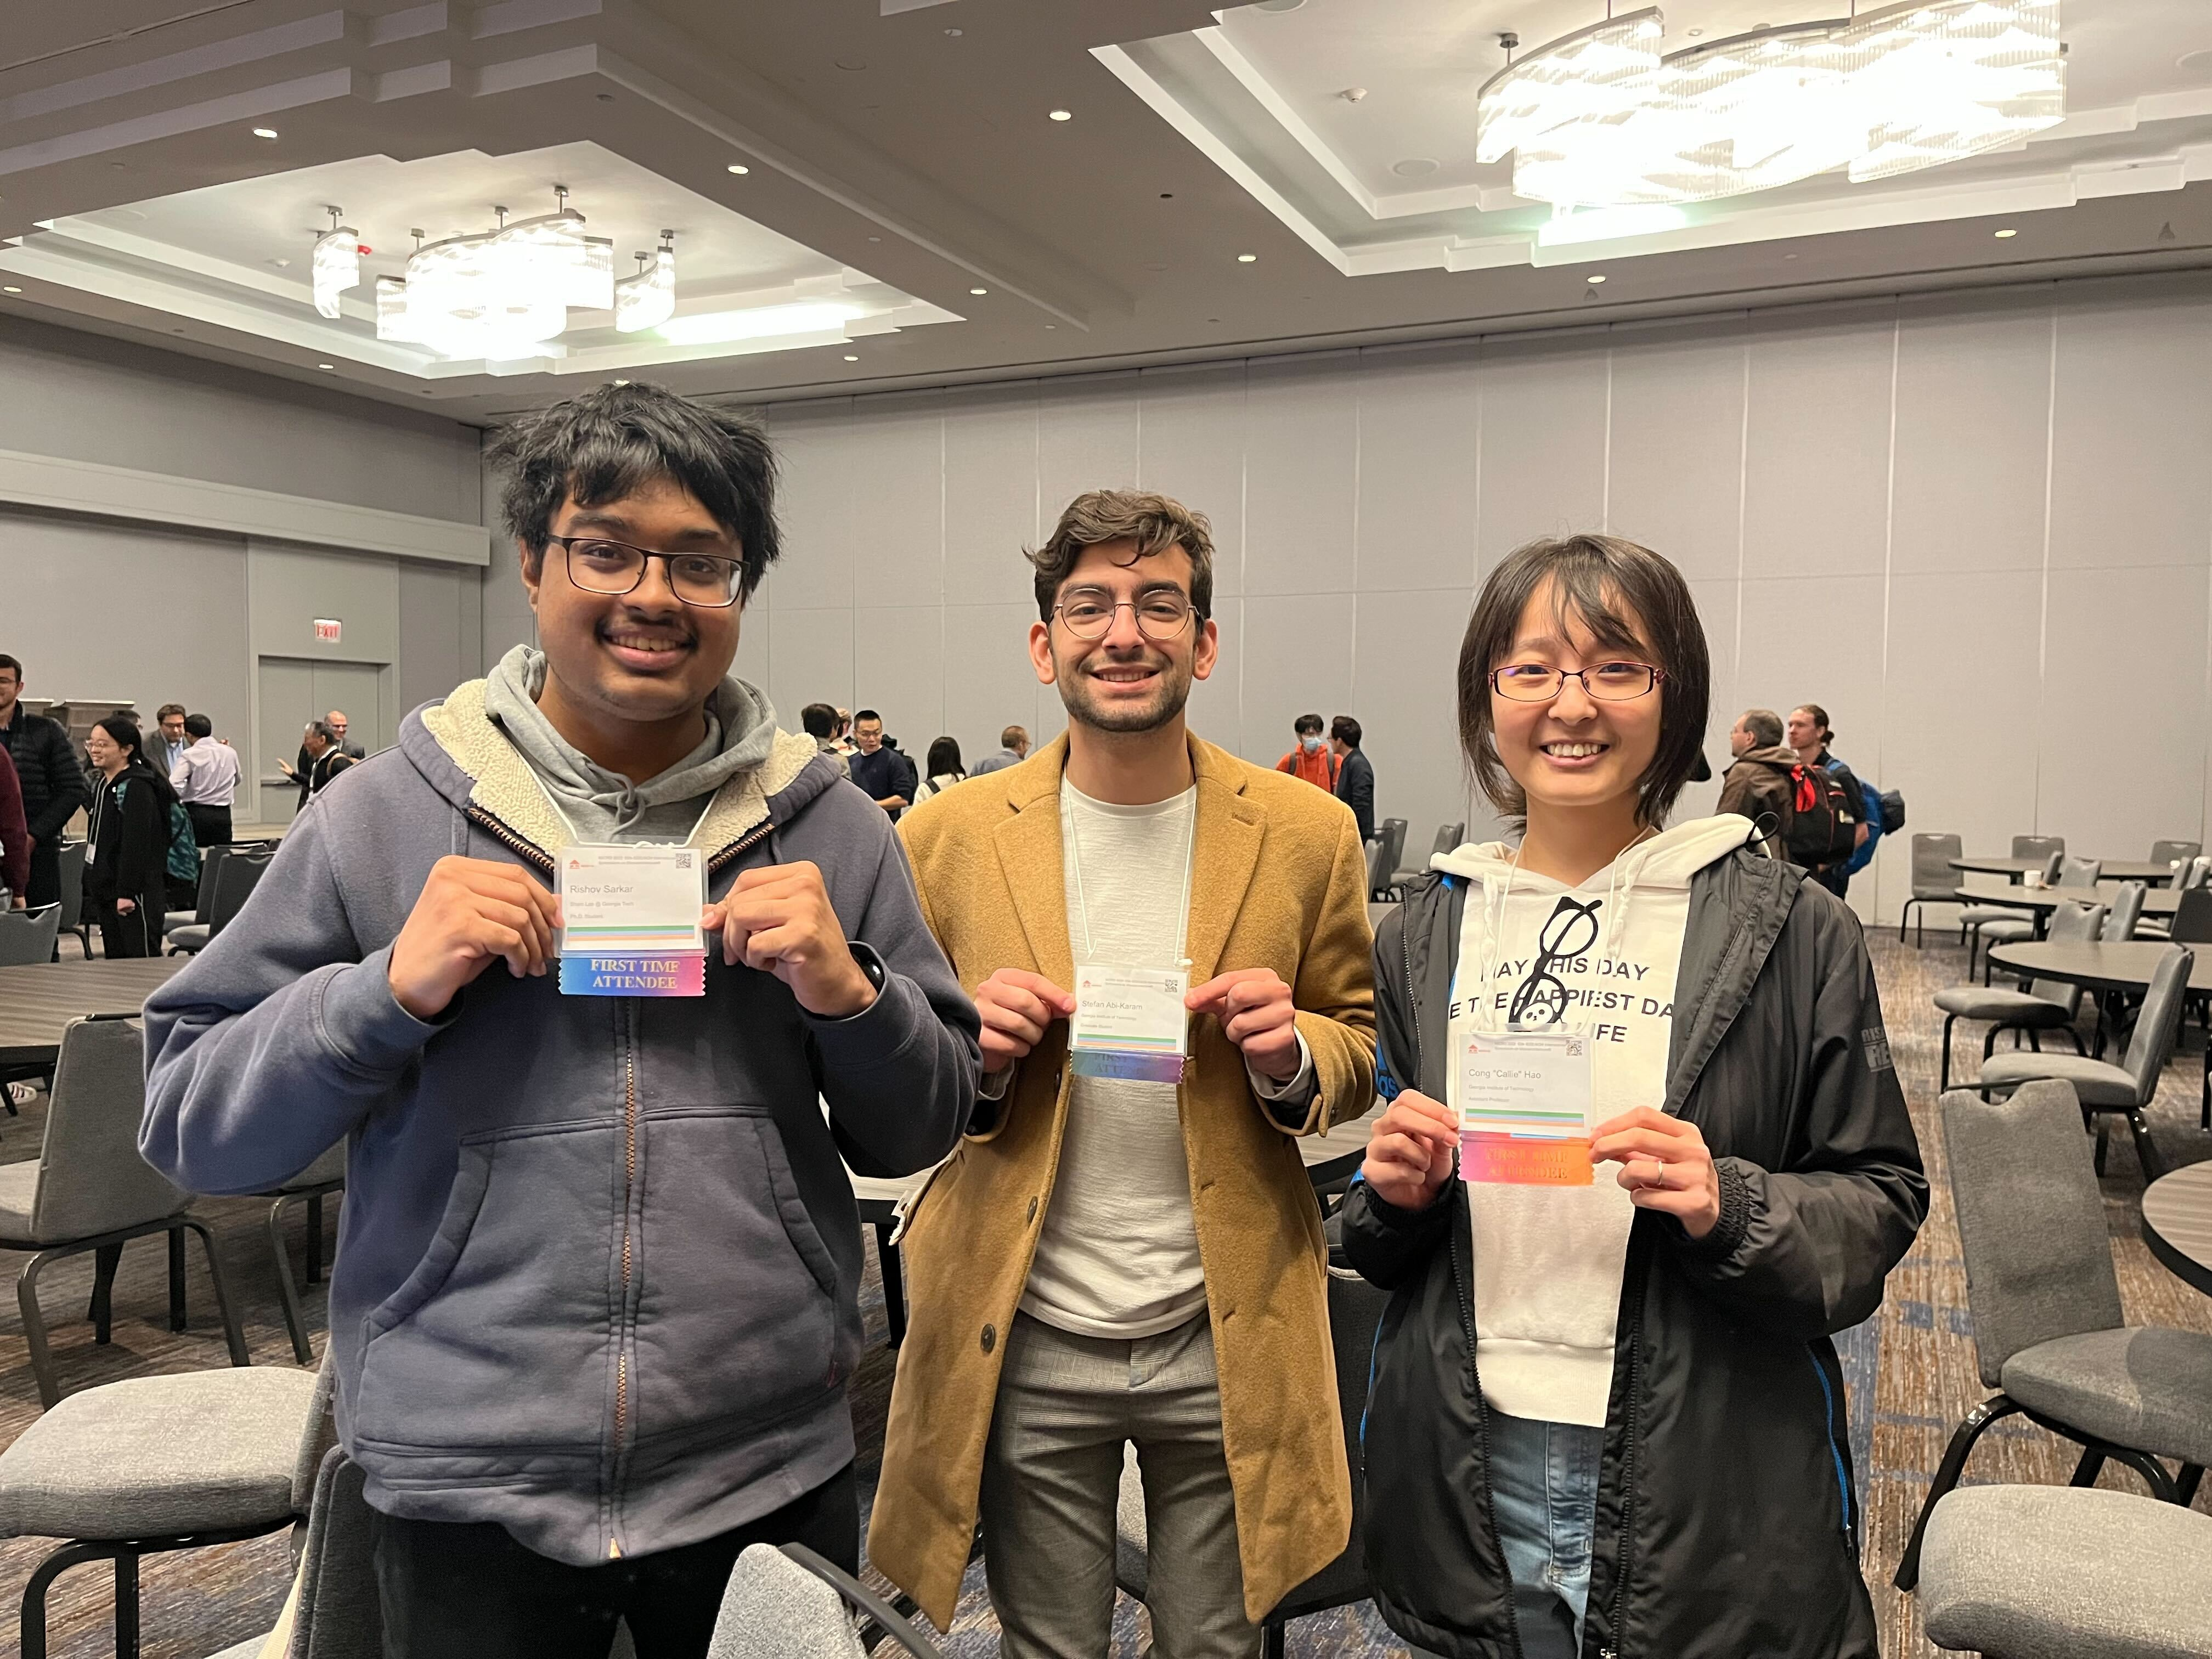
\includegraphics[width=0.8\textwidth]{imgs/me_2.jpg}
        \end{column}
    \end{columns}
\end{frame}

\begin{frame}{About Your Teacher}

    \textbf{More Details}
    \begin{itemize}
        \item \href{https://sharclab.ece.gatech.edu/}{SHARC Lab, ECE, Georgia Tech}
              % \item CIPHER Lab, Georgia Tech Research Institute
        \item \href{https://www.gtri.gatech.edu/laboratories/cybersecurity-information-protection-and-hardware-evaluation-research}{CIPHER Lab, Georgia Tech Research Institute}
              % \item Georgia Tech Undergraduate Admissions
        \item \href{https://admission.gatech.edu/}{Georgia Tech Undergraduate Admissions}
    \end{itemize}

    \vspace{\baselineskip}

    \textbf{Hobbies}
    \begin{itemize}
        \item Meteorology
        \item Music Production and Analog Music Synthesis
        \item Sailing
        \item Hobby Electronics and Programming
        \item Reading
    \end{itemize}

\end{frame}

\begin{frame}{About Your Teacher}
    \centering
    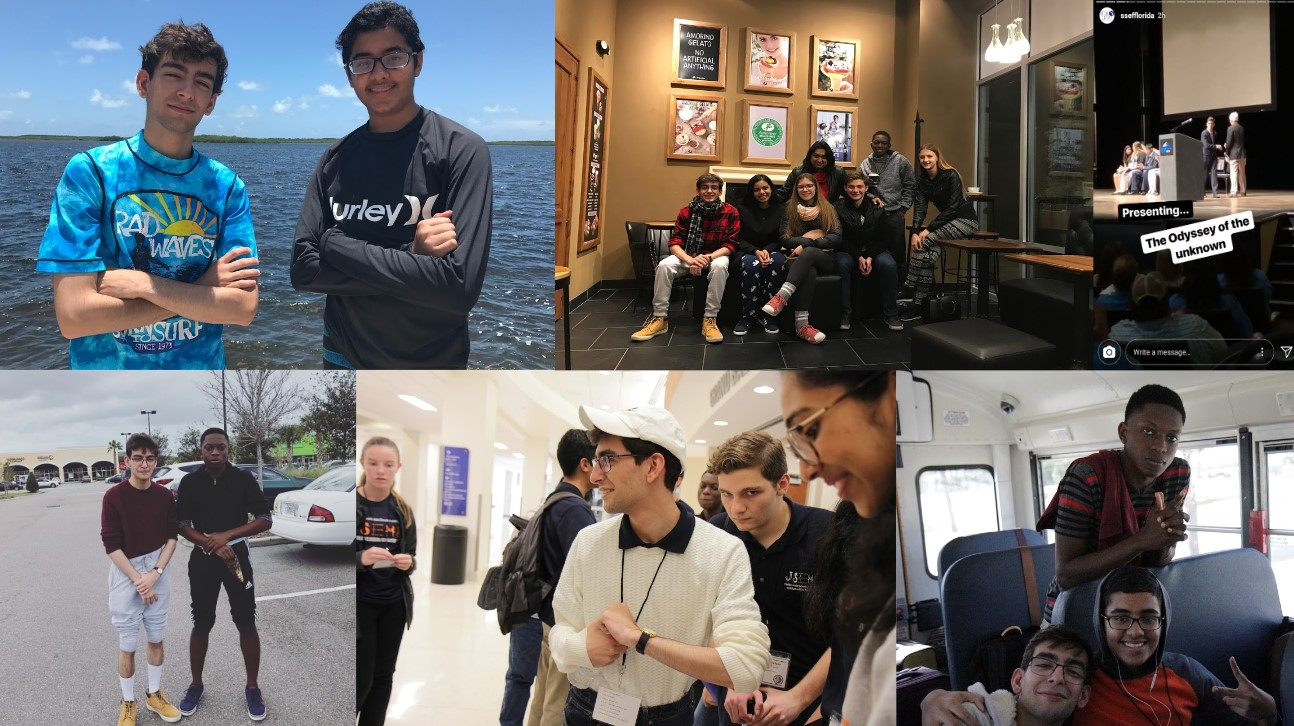
\includegraphics[width=0.9\textwidth]{imgs/me_3.jpg}
\end{frame}


\section{Scientific Computing Overview}

\begin{frame}{What is Computing?}

    \begin{quote}
        Computer Science is no more about computers than astronomy is about telescopes.
        \begin{flushleft}
            ---Edsger W. Dijkstra
        \end{flushleft}
    \end{quote}

\end{frame}

\begin{frame}{Scientific Computing - Earth Science and Engineering}
    \centering
    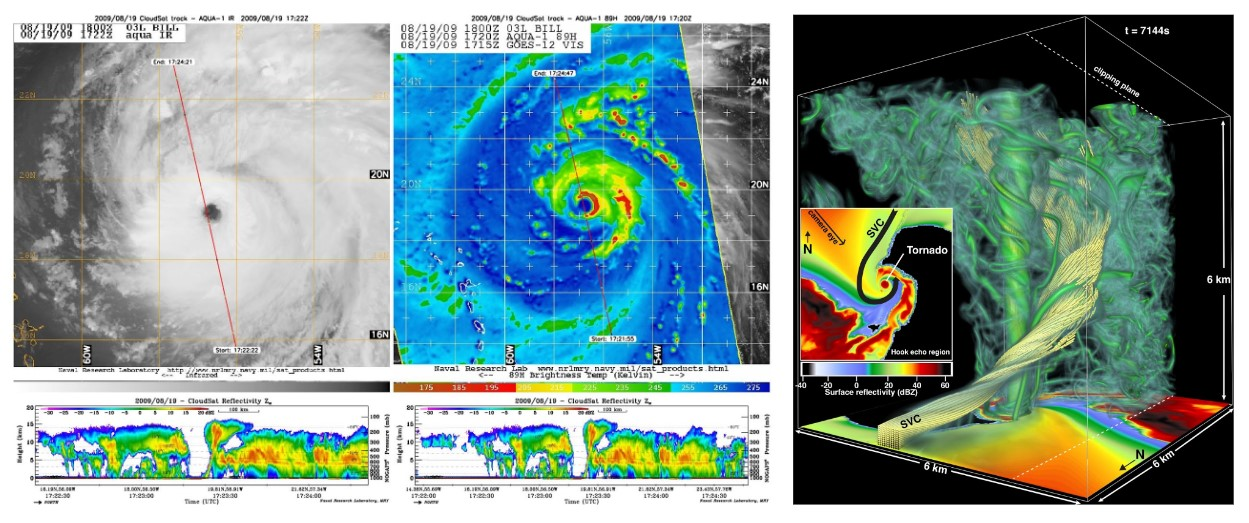
\includegraphics[width=0.7\textwidth]{imgs/vis_0.jpg}
    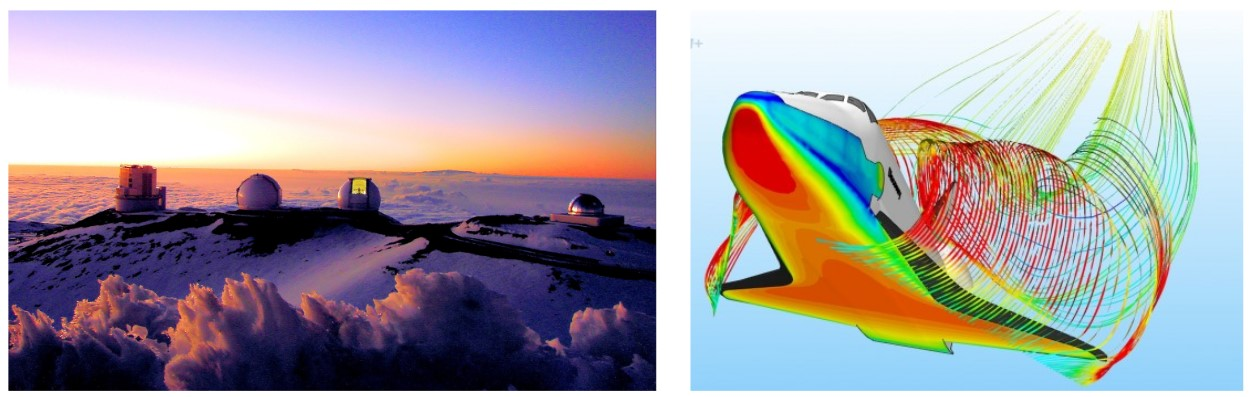
\includegraphics[width=0.7\textwidth]{imgs/vis_1.jpg}
\end{frame}

\begin{frame}{Scientific Computing - Biology and Medicine}
    \centering
    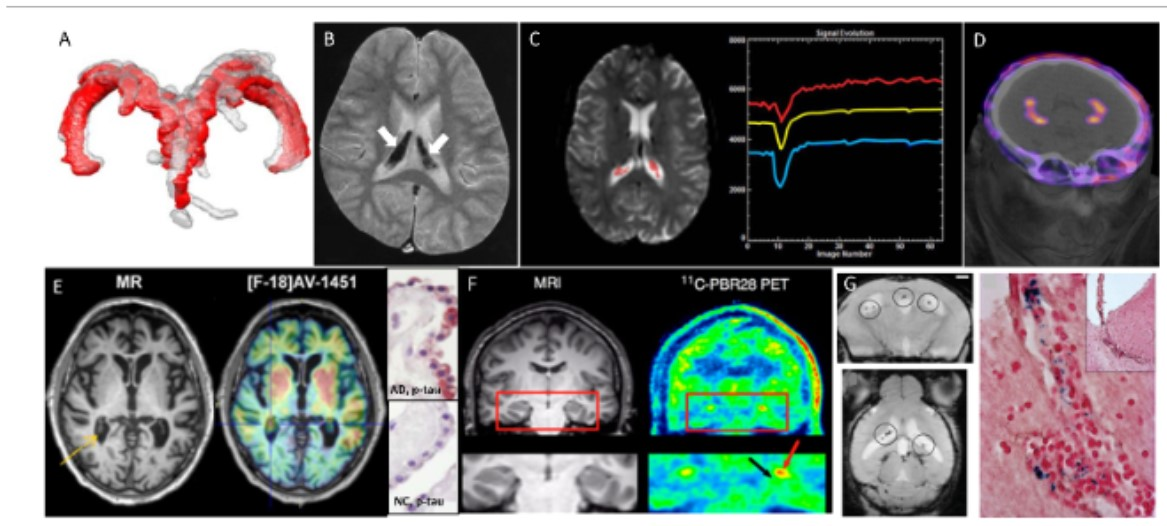
\includegraphics[width=0.65\textwidth]{imgs/vis_2.jpg}
    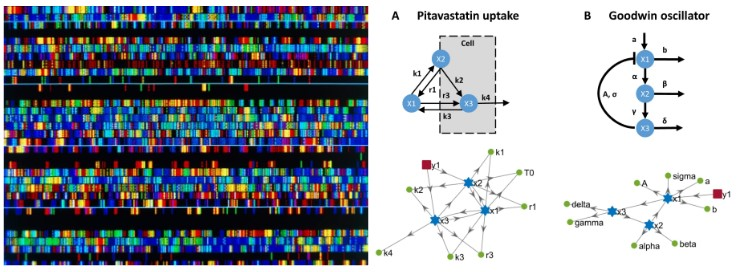
\includegraphics[width=0.65\textwidth]{imgs/vis_3.jpg}
\end{frame}

\begin{frame}{What is Data Science?}
    \begin{quote}
        Data is the new oil.
    \end{quote}
\end{frame}

\begin{frame}{Data Science - COVID-19}
    \centering
    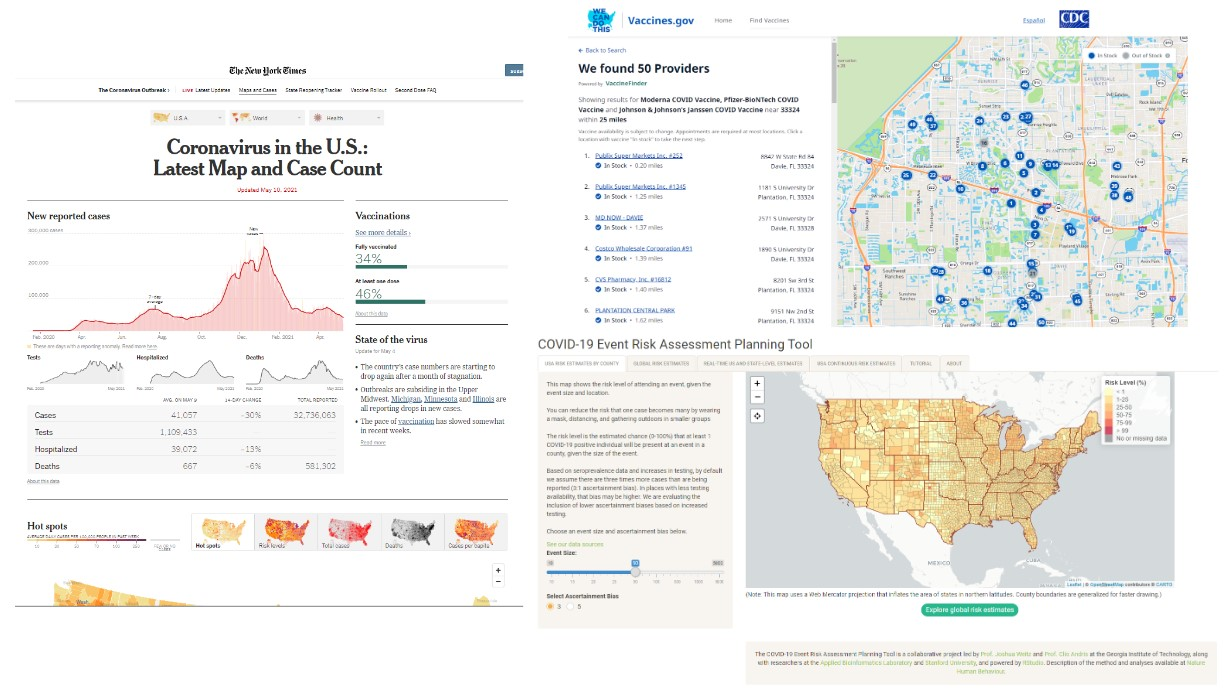
\includegraphics[width=0.9\textwidth]{imgs/vis_4.jpg}
\end{frame}

\begin{frame}{Data Science - General Applications}
    \centering
    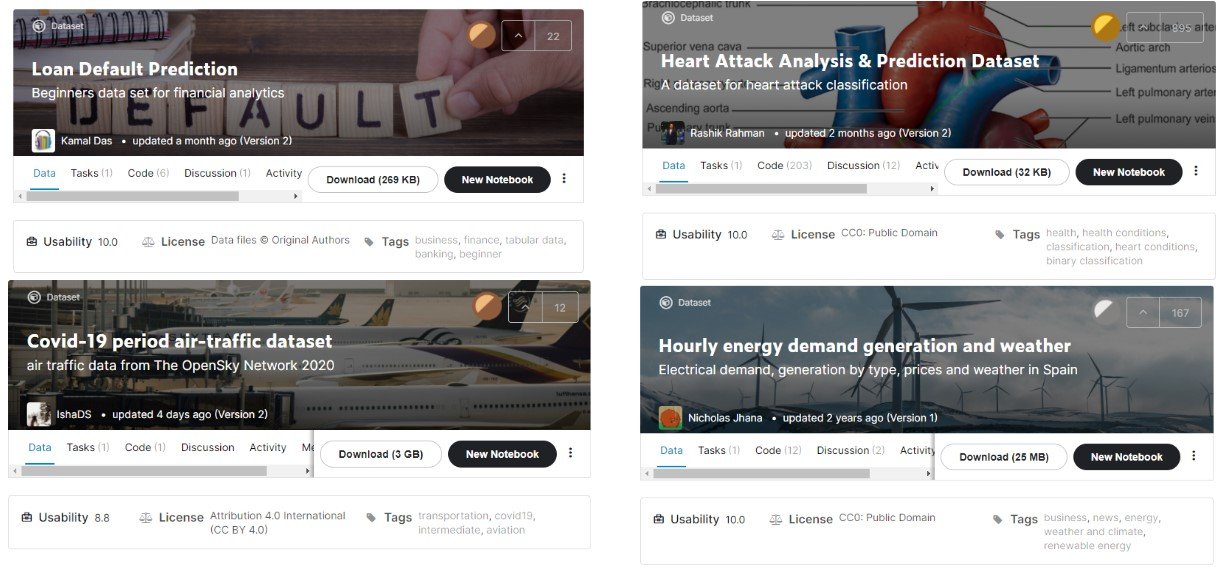
\includegraphics[width=\textwidth]{imgs/vis_5.jpg}
\end{frame}

\begin{frame}{What is Machine Learning?}
    \begin{quote}
        AI is the new electricity.
        \begin{flushleft}
            ---Andrew Ng
        \end{flushleft}
    \end{quote}

    \vspace{\baselineskip}

    In the same way that electricity transformed our world, AI will transform our world and will be incorporated into every aspect of our lives.

\end{frame}


\begin{frame}{AI vs. Machine Learning vs. Deep Learning}

    \begin{columns}
        \begin{column}{0.5\textwidth}
            \begin{itemize}
                \item \textbf{AI:} The study of how to make computers intelligent.
                \item \textbf{Machine Learning:} A subfield of computer science that gives computers the ability to learn without being explicitly programmed.
                \item \textbf{Deep Learning:} A subfield of machine learning that uses neural-network-like structures and large amounts of data to learn.
            \end{itemize}
        \end{column}
        \begin{column}{0.5\textwidth}
            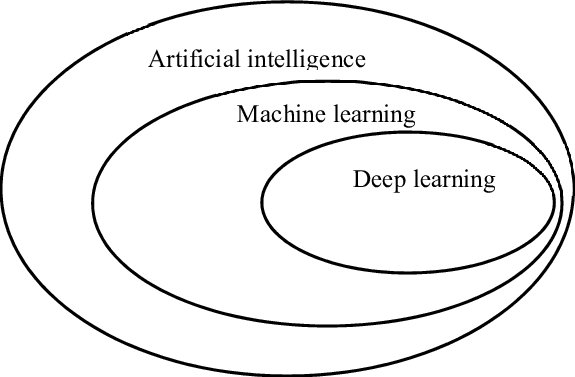
\includegraphics[width=\textwidth]{imgs/ai_diagram.jpg}
        \end{column}
    \end{columns}

\end{frame}

\begin{frame}{Machine Learning - Self-Driving Cars}
    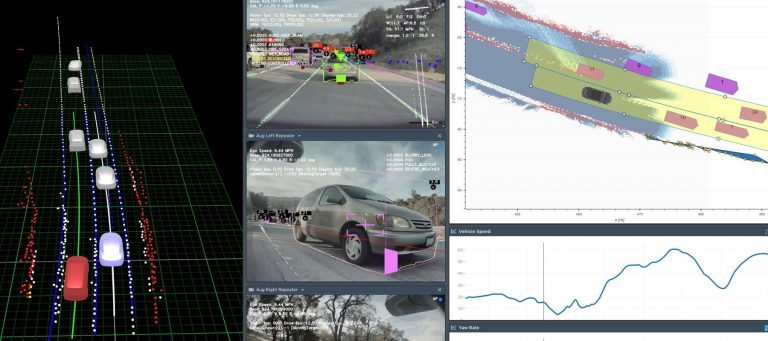
\includegraphics[width=\textwidth]{imgs/vis_6.jpg}
\end{frame}

\begin{frame}{Machine Learning - Generative Models}
    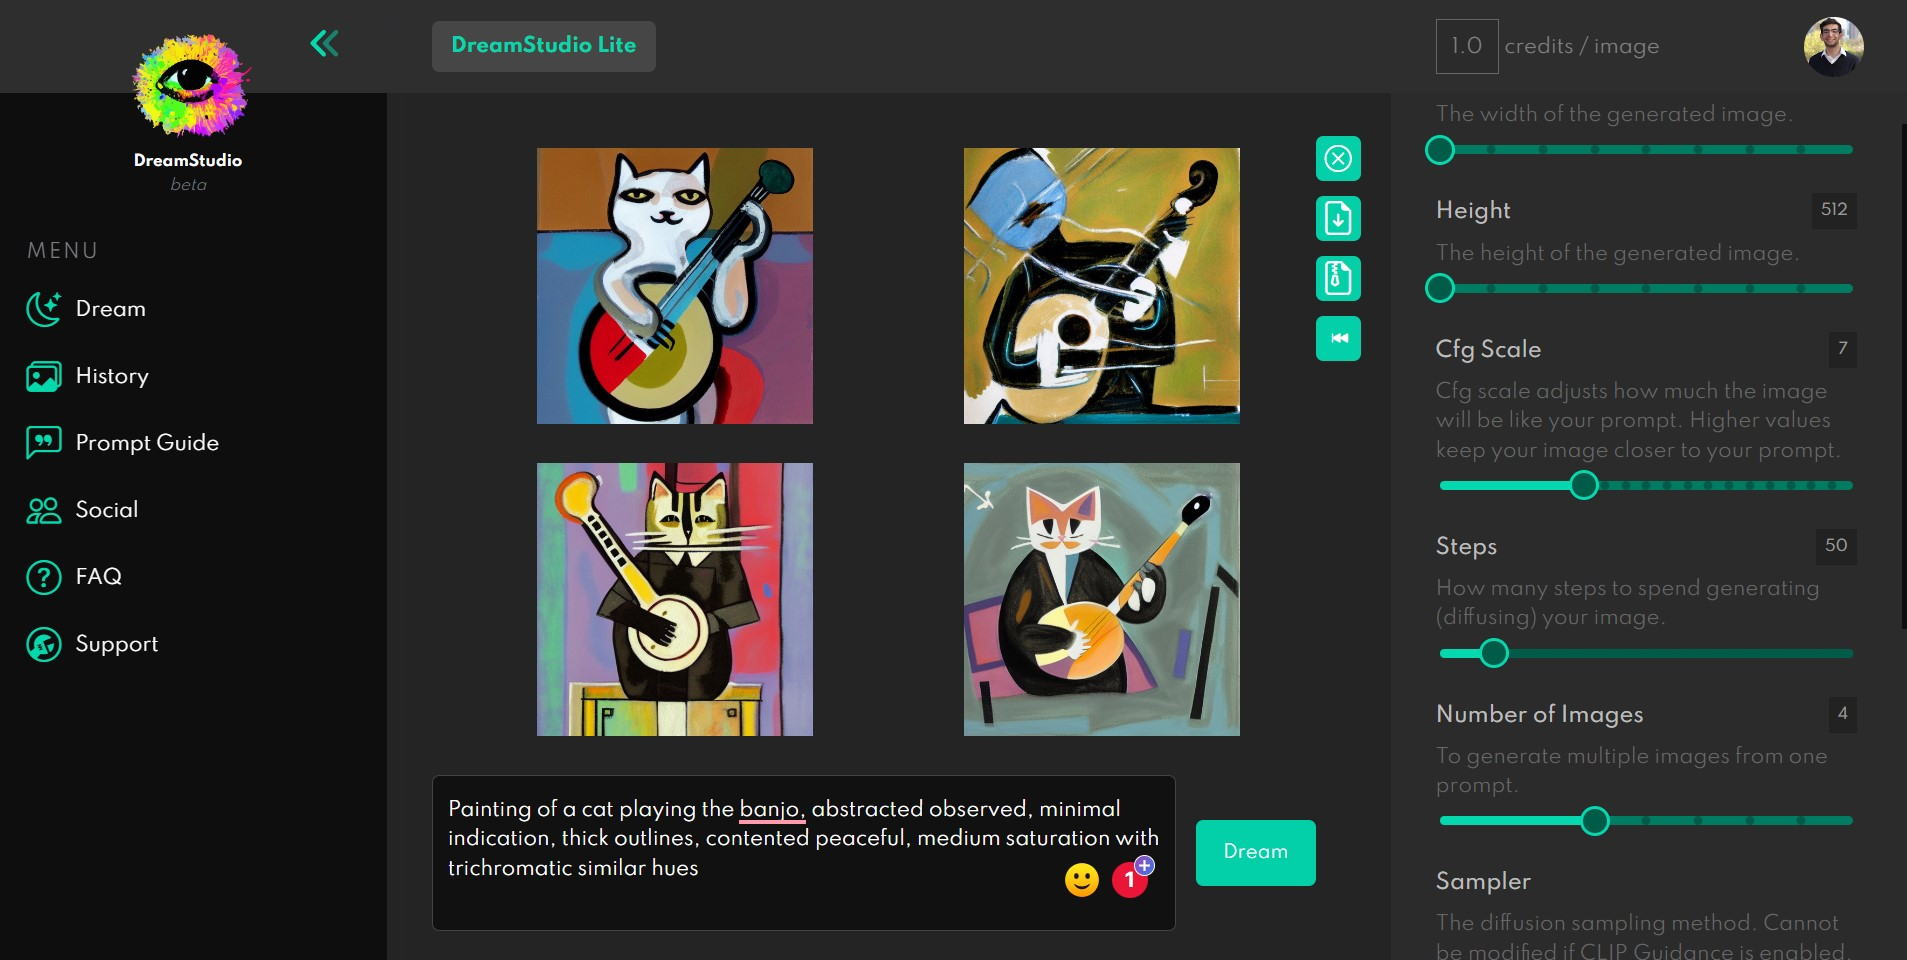
\includegraphics[width=\textwidth]{imgs/vis_7.jpg}
\end{frame}


\begin{frame}{Machine Learning - Protien Folding}
    \centering
    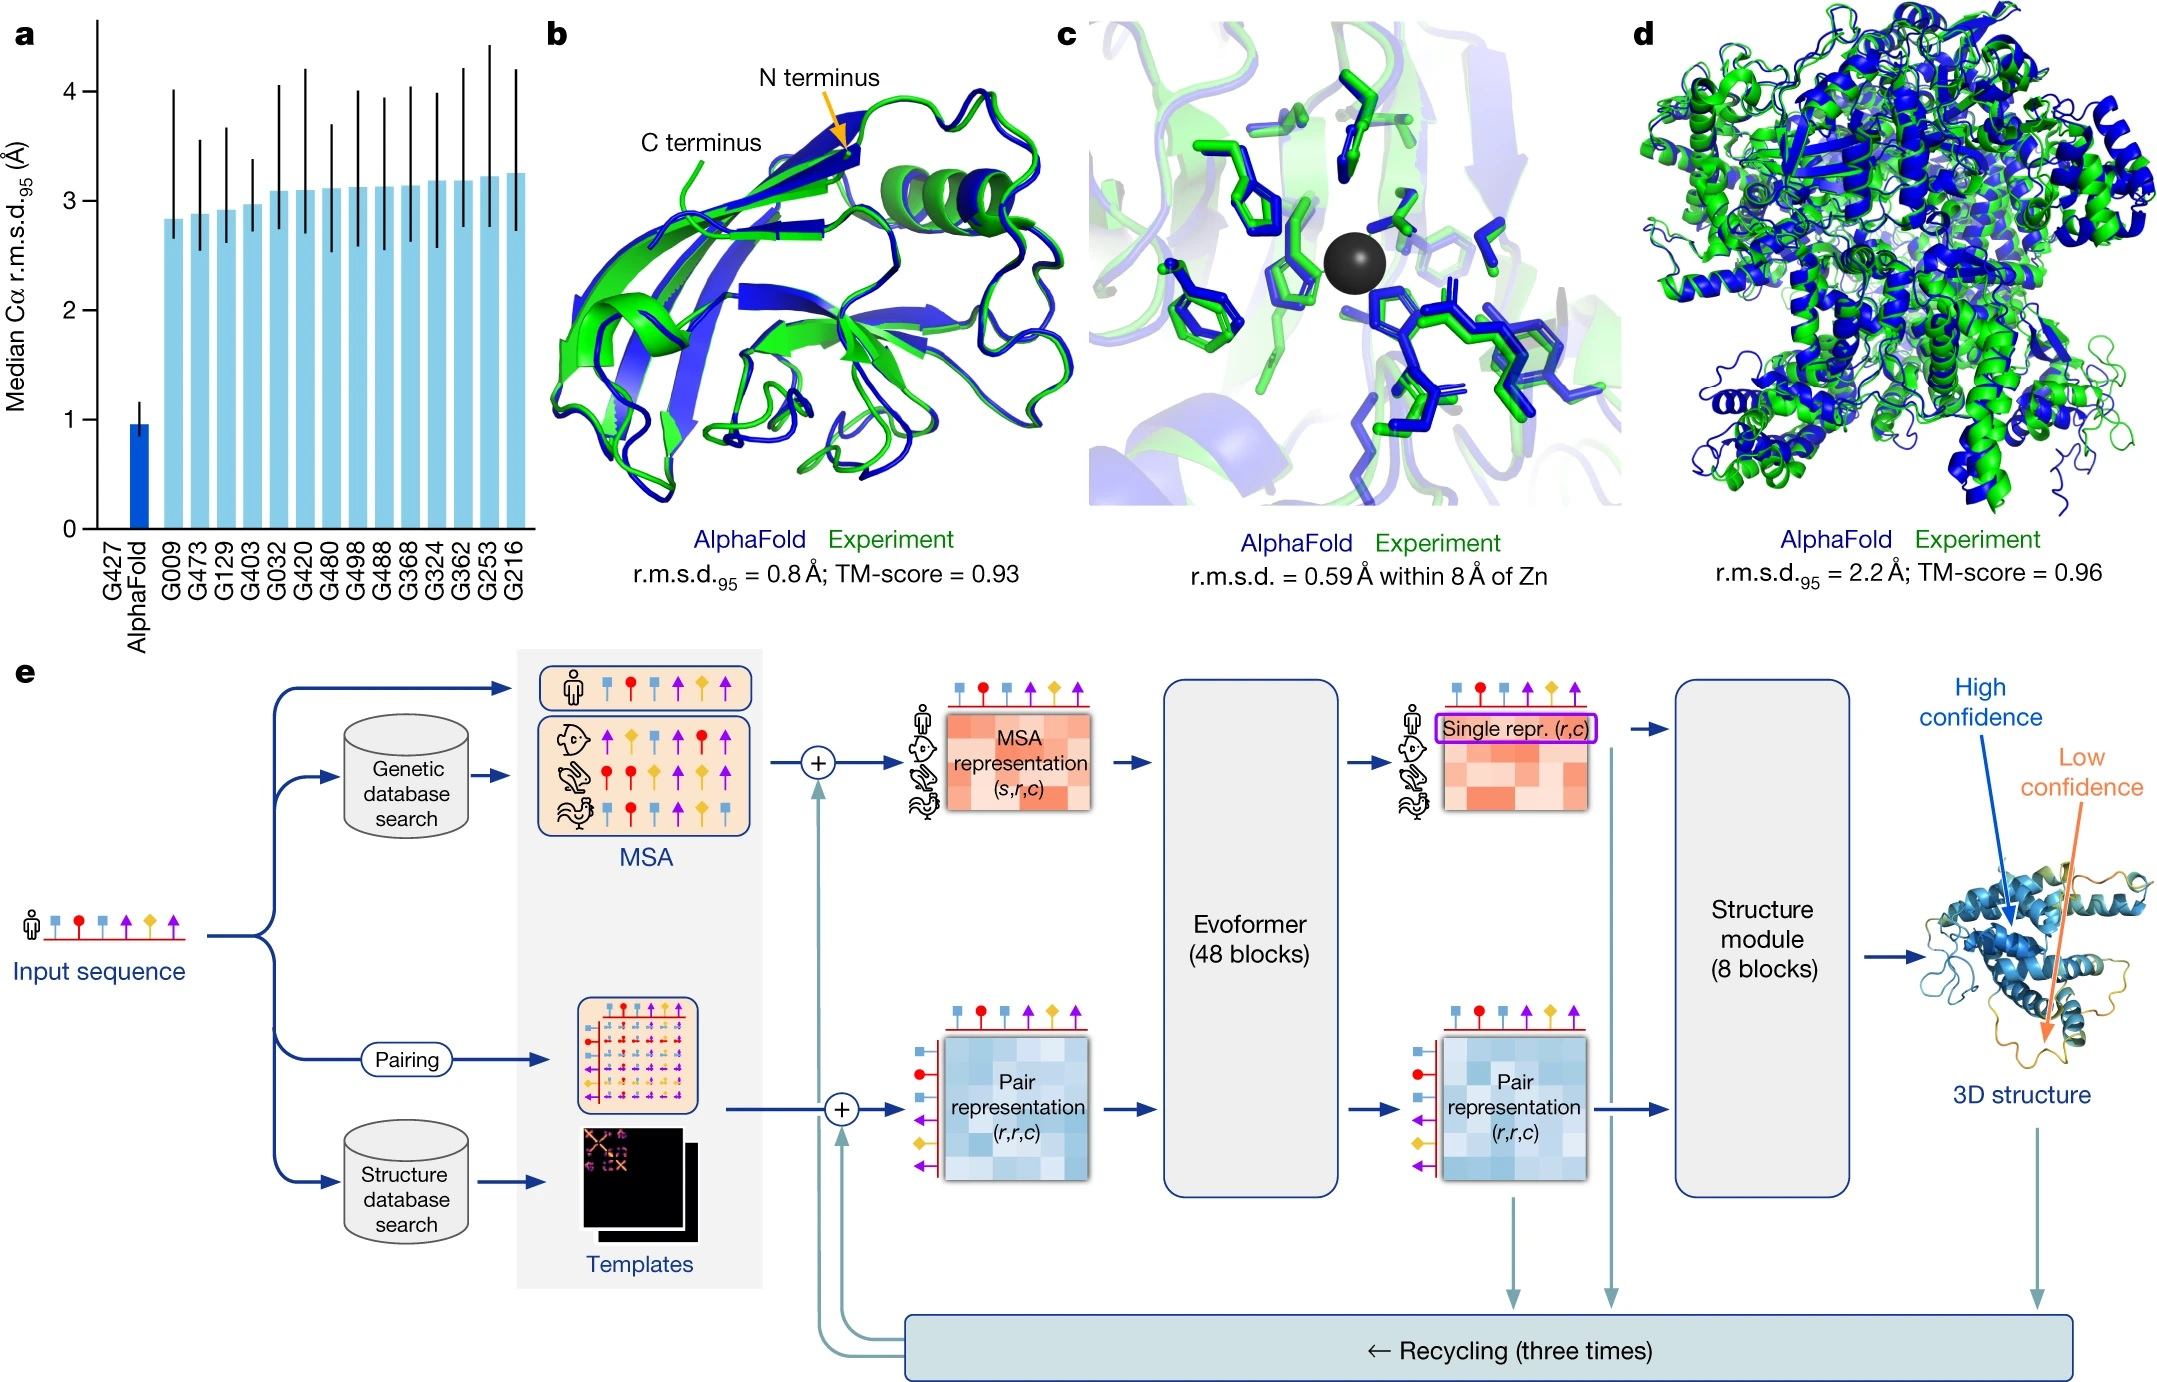
\includegraphics[width=0.8\textwidth]{imgs/vis_9.jpg}
\end{frame}

\begin{frame}{Machine Learning - Protien Folding}
    \centering
    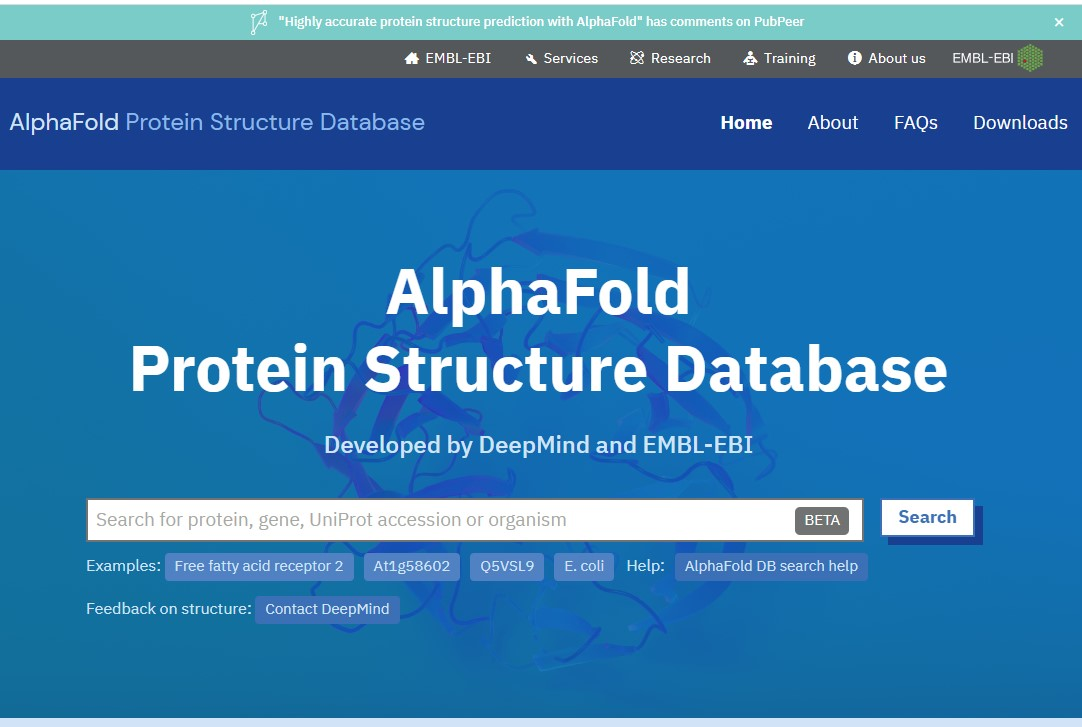
\includegraphics[width=0.8\textwidth]{imgs/vis_8.jpg}
\end{frame}

\section{Closing Advice}

\begin{frame}{Closing Advice}
    \begin{itemize}
        \item Find connections between your interest and what we will cover and explore those connections; always keep that in the back of your mind.
        \item There is no such thing as a dumb question; if you have a question or a gap in your understanding, ask about it as soon as possible.
        \item I am flexible about a lot of things if you come to me early and talk to me directly.
        \item I have a good sense of humor, so any class or research memes are encouraged.
    \end{itemize}
\end{frame}

\end{document}